\let\negmedspace\undefined
\let\negthickspace\undefined
\documentclass[journal]{IEEEtran}
\usepackage[a5paper, margin=10mm, onecolumn]{geometry}
%\usepackage{lmodern} % Ensure lmodern is loaded for pdflatex
\usepackage{tfrupee} % Include tfrupee package

\setlength{\headheight}{1cm} % Set the height of the header box
\setlength{\headsep}{0mm}     % Set the distance between the header box and the top of the text

\usepackage{gvv-book}
\usepackage{gvv}
\usepackage{cite}
\usepackage{amsmath,amssymb,amsfonts,amsthm}
\usepackage{algorithmic}
\usepackage{graphicx}
\usepackage{textcomp}
\usepackage{xcolor}
\usepackage{txfonts}
\usepackage{listings}
\usepackage{enumitem}
\usepackage{mathtools}
\usepackage{gensymb}
\usepackage{comment}
\usepackage[breaklinks=true]{hyperref}
\usepackage{tkz-euclide} 
\usepackage{listings}
% \usepackage{gvv}                                        
\def\inputGnumericTable{}                                 
\usepackage[latin1]{inputenc}                                
\usepackage{color}                                            
\usepackage{array}                                            
\usepackage{longtable}                                       
\usepackage{calc}                                             
\usepackage{multirow}                                         
\usepackage{hhline}                                           
\usepackage{ifthen}                                           
\usepackage{lscape}
\begin{document}

\bibliographystyle{IEEEtran}
\vspace{3cm}

\title{1.9.12}
\author{EE24BTECH11001 - Aditya Tripathy
}
 \maketitle
% \newpage
% \bigskip
{\let\newpage\relax\maketitle}

\renewcommand{\thefigure}{\theenumi}
\renewcommand{\thetable}{\theenumi}
\setlength{\intextsep}{10pt} % Space between text and floats


\numberwithin{equation}{enumi}
\numberwithin{figure}{enumi}
\renewcommand{\thetable}{\theenumi}


\textbf{Question}:\\
Find the length of the segment joining $\vec{A}\brak{-6,7}$ and $\vec{B}\brak{-1,-5}$. Also, find the midpoint of $\vec{AB}$.
\\
\textbf{Solution: }\\
From \brak{1.1.7.1}, length of vector X is given by
\begin{align} 
    ||\vec{X}|| = \sqrt{\vec{X}^\top \vec{X}}
\end{align}
\begin{align}
    \vec{X} = \vec{B} - \vec{A} = \myvec{-1 \\ -5} - \myvec{-6 \\ 7} = \myvec{5 \\ -12}\\
    ||\vec{X}|| = \sqrt{\myvec{5 & -12}\myvec{5 \\ -12}} = \sqrt{25 + 144} = 13.\\
\end{align}
The length of the given vector = 13.\\
From \brak{1.1.4.1}, the point dividing $\vec{BC}$ in ratio $k:1$ is given by,
\begin{align}
    \vec{D} = \frac{k\vec{C}+\vec{B}}{k+1}\\
\end{align}
\begin{align}
    \vec{D} = \frac{\vec{B}+\vec{A}}{1+1} \\
    \vec{D} = \myvec{-3.5 \\ 1}
\end{align}
    
\begin{figure}[h!]
   \centering
   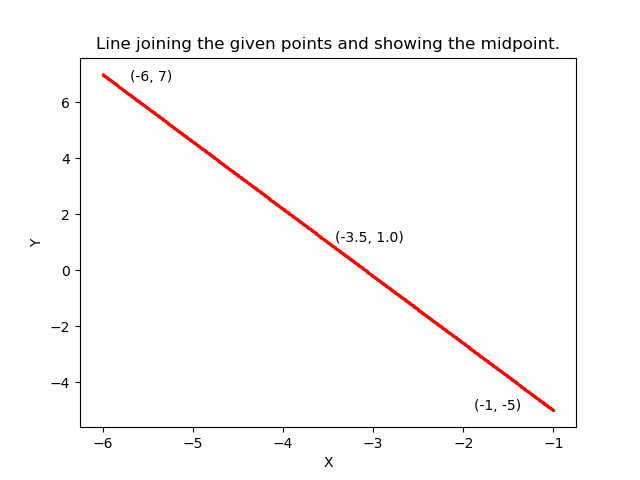
\includegraphics[width=0.7\linewidth]{figs/fig.png}
   \caption{Line joining the given points and the midpoint}
\end{figure}
\end{document}  
